% Why landmarks are priced rather than counted: one action achieving two of them.
\documentclass[tikz,border=0pt]{standalone}
\usepackage{amsmath}
\usepackage{tikz}
\usetikzlibrary{backgrounds,arrows.meta,positioning}
\definecolor{hdblue}{HTML}{1B4F8A}
\definecolor{hdred}{HTML}{A62B1F}
\begin{document}
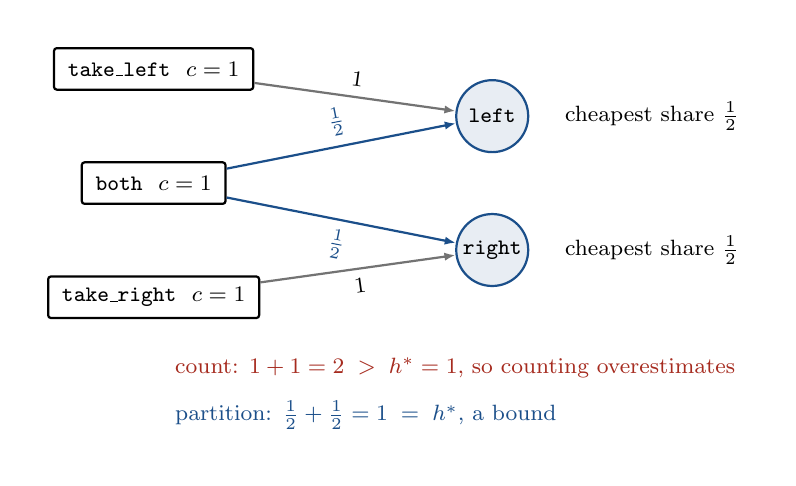
\begin{tikzpicture}[
    show background rectangle, inner frame sep=7pt,
    background rectangle/.style={fill=white},
    font=\footnotesize, >={Latex[length=4pt]},
    act/.style={rectangle,draw=black,thick,fill=white,rounded corners=1pt,
                minimum height=15pt,inner xsep=5pt},
    lm/.style={circle,draw=hdblue,thick,fill=hdblue!10,minimum size=26pt,inner sep=1pt},
    share/.style={->,hdblue,thick},
    weak/.style={->,black!55,thick}]

  \node[act] (tl) at (0, 1.45) {\texttt{take\_left}\ \ $c=1$};
  \node[act] (bo) at (0, 0.00) {\texttt{both}\ \ $c=1$};
  \node[act] (tr) at (0,-1.45) {\texttt{take\_right}\ \ $c=1$};

  \node[lm] (l) at (4.3, 0.85) {\texttt{left}};
  \node[lm] (r) at (4.3,-0.85) {\texttt{right}};

  \draw[weak]  (tl) -- node[above,sloped,pos=0.5,black] {$1$}   (l);
  \draw[weak]  (tr) -- node[below,sloped,pos=0.5,black] {$1$}   (r);
  \draw[share] (bo) -- node[above,sloped,pos=0.5,hdblue] {$\tfrac{1}{2}$} (l);
  \draw[share] (bo) -- node[below,sloped,pos=0.5,hdblue] {$\tfrac{1}{2}$} (r);

  \node[anchor=west,align=left] at (5.1,0.85) {cheapest share $\tfrac{1}{2}$};
  \node[anchor=west,align=left] at (5.1,-0.85) {cheapest share $\tfrac{1}{2}$};

  \node[hdred,  anchor=west] at (0.15,-2.35)
       {count: $1 + 1 = 2 \;>\; h^{*} = 1$, so counting overestimates};
  \node[hdblue, anchor=west] at (0.15,-2.95)
       {partition: $\tfrac{1}{2} + \tfrac{1}{2} = 1 \;=\; h^{*}$, a bound};
\end{tikzpicture}
\end{document}
